\documentclass{article}
\usepackage{fancyhdr} % for pretty formatting
\usepackage{amsmath} % for matrices
\usepackage{amssymb} % for bold text
\usepackage{pgfplots} % for graphs
\usepackage{hyperref} % for hyperlinks
\pgfplotsset{compat=1.18}

\usepackage{lipsum} % For dummy text
\usepackage{cite} % For citations

\pagestyle{fancy}
\fancyhf{} % Clear all header and footer fields

\lhead{Joshua Dunne}
\rhead{\thepage} % Displays the current page number
\lfoot{MATH620}
\cfoot{Homework 1}

\begin{document}
\section{Question 1}
    \subsection{Consider}
    \begin{center}
    $4 \begin{bmatrix}1 \\ -3 \end{bmatrix}$ and $-2 \begin{bmatrix}3 \\ 5 \end{bmatrix}$
    \end{center}


    \subsection{Graphical representation unscaled}
        \begin{minipage}{0.49\textwidth}
            \centering
            \begin{tikzpicture}
                \begin{axis}[
                    width=\linewidth,
                    title={1, -3},
                    xmin= -7, xmax=7,
                    ymin=-7, ymax=7
                ]
                \addplot[blue, smooth, mark=*] coordinates {
                    (0,0) (1, -3)
                };
                \end{axis}
            \end{tikzpicture}
            \label{fig:graph1}
        \end{minipage}
        \hfill % Add a horizontal space between the graphs
        % Start of second minipage
        \begin{minipage}{0.49\textwidth}
            \centering
            \begin{tikzpicture}
                \begin{axis}[
                    width=\linewidth,
                    title={3, 5},
                    xmin= -7, xmax=7,
                    ymin=-7, ymax=7
                ]
                \addplot[red, smooth, mark=*] coordinates {
                    (0,0) (3,5)
                };
                \end{axis}
            \end{tikzpicture}
        \end{minipage}%


    \subsection{Graphical representation scaled}
        \begin{minipage}{0.49\textwidth}
        \centering
        \begin{tikzpicture}
            \begin{axis}[
                width=\linewidth,
                title={4 * (1, -3)},
                xmin= -13, xmax=13,
                ymin=-13, ymax=13
            ]
            \addplot[blue, smooth, mark=*] coordinates {
                (0,0) (4, -12)
            };
            \end{axis}
        \end{tikzpicture}
    \end{minipage}
    \hfill % Add a horizontal space between the graphs
    % Start of second minipage
    \begin{minipage}{0.49\textwidth}
        \centering
        \begin{tikzpicture}
            \begin{axis}[
                width=\linewidth,
                title={-2 * (3, 5)},
                xmin= -13, xmax=13,
                ymin=-13, ymax=13
            ]
            \addplot[red, smooth, mark=*] coordinates {
                (0,0) (-6,-10)
            };
            \end{axis}
        \end{tikzpicture}
    \end{minipage}%


    \subsection{Added together}
        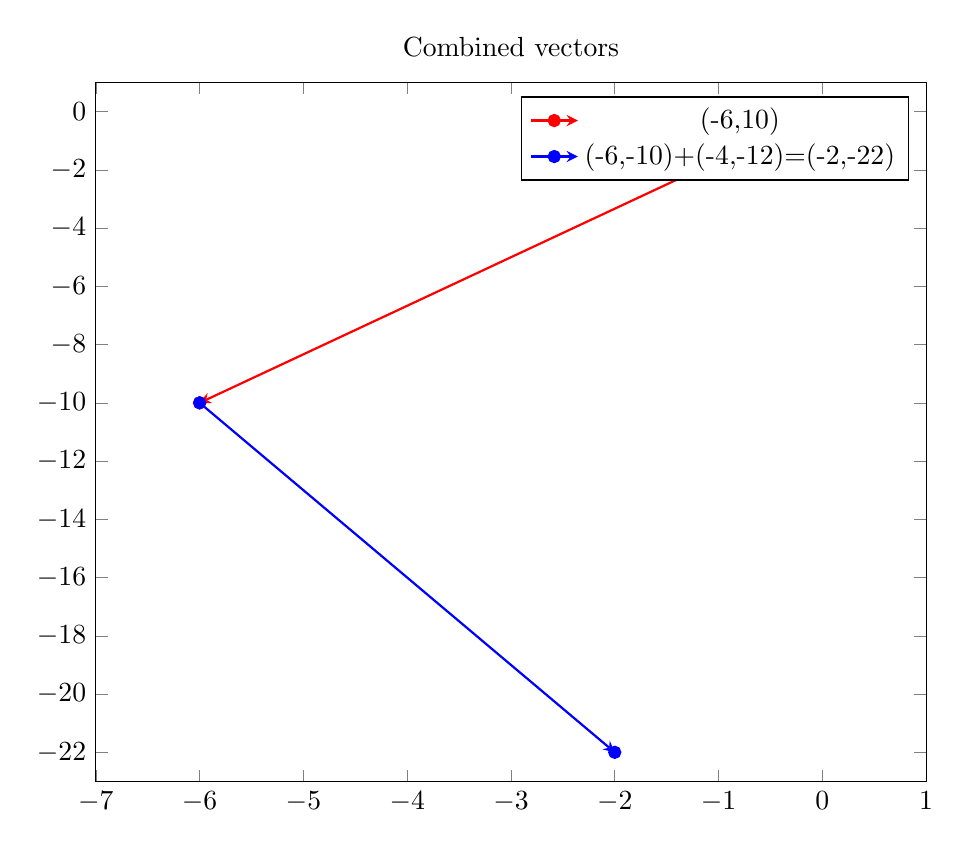
\begin{tikzpicture}
            \begin{axis}[
                width=\linewidth,
                title={Combined vectors},
                xmin= -7, xmax=1,
                ymin=-23, ymax=1
            ]
            \addplot[red, smooth, mark=*, -stealth, thick] coordinates {
                (0,0) (-6,-10)
            };
            \addlegendentry{(-6,10)}
            \addplot[blue, smooth, mark=*, -stealth, thick] coordinates {
                (-6,-10) (-2, -22)
            };
            \addlegendentry{(-6,-10)+(-4,-12)=(-2,-22)}
            \end{axis}
        \end{tikzpicture}
    \subsection{Changes}
    As can be seen in the graphs above. The coefficient before each of the column
    matrices can be seen to scale any offset. For example, were we to take negative
    one times a matrix, then the offset would extend as far in the negative directions
    as a matrix extended in the positives. When we scale them by a multiplier and then add
    (subtract) from one another.





\section{Question 2}
    \subsection{Quick reiteration}
    Having found that we were unable to reach old man Gauss's house using only
    one form of transport, justify this conclusion with two approaches.


    \subsection{First approach}
    \paragraph{Induction}
        For this to be true we'd, much like before, need a coefficient with which
        we'd be able to multiply by our column vector to get to $\begin{bmatrix}107 \\ 64\end{bmatrix}$
        \[{c_1}\begin{bmatrix}3 \\ 1\end{bmatrix} = \begin{bmatrix}107 \\ 64\end{bmatrix}\]
        \[{c_2}\begin{bmatrix}1 \\ 2\end{bmatrix} = \begin{bmatrix}107 \\ 64\end{bmatrix}\]
        However, there simply are not $c_1$ or $c_2$ $\in{\mathbb{R}}$ that satisfy either equation.
        It is therefor impossible to reach his home.


    \subsection{Second approach}
    \paragraph{Visual}
        We can illustrate this as a form of argument. As $\begin{bmatrix}3 \\ 1\end{bmatrix}$ forms a line
        $y=\frac{3}{1}x+0$ That is, by scaling, we can point the end of this vector
        to any point on the line defined. However $(107, 64)$ is not on that line. No possible scaling
        could result in a point that is not on the line.
        \begin{center}
        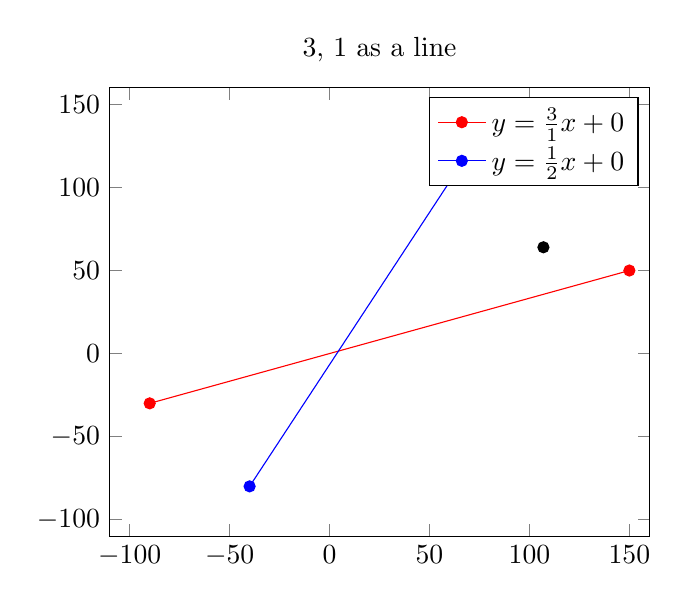
\begin{tikzpicture}
            \begin{axis}[
                title={3, 1 as a line},
                xmin= -110, xmax=160,
                ymin=-110, ymax=160
            ]
            \addplot[red, smooth, mark=*] coordinates { (-90,-30) (150,50) };
            \addlegendentry{$y=\frac{3}{1}x+0$}
            \addplot[blue, smooth, mark=*] coordinates { (-40,-80) (80,140) };
            \addlegendentry{$y=\frac{1}{2}x+0$}
            \addplot[only marks, mark=*] coordinates { (107,64) };
            \end{axis}
        \end{tikzpicture}
        \end{center}
    \paragraph{Analysis}
    As can be seen as depicted, either vector, when scaled, is insufficient
    to reach the point. It is only when we combine the two that we can reach
    both old man Gauss's house and the entirety of $\mathbb{R}^2$





\section{Question 3}
    \subsection{Quick reiteration}
        \paragraph{Introduction}We \emph{want} to show that given vectors $\vec{b_1}$ and $\vec{b_2}$ 
        where $\vec{b_1}=\begin{bmatrix}3\\1\end{bmatrix}$ and $\vec{b_2}=\begin{bmatrix}1\\2\end{bmatrix}$
        can be taken in a linear combination to form $\mathbb{R}^2$. \emph{If} this were the case then we could expect
        that given any combination $r_1$, $r_2$ $\in \mathbb{R}$ would have solutions\\ $c_1, c_2$ $\in \mathbb{R}$ such that
        $c_1\vec{b_1}+c_2\vec{b_2}=\begin{bmatrix}r_1\\r_2\end{bmatrix}$
        \paragraph{Method}To show this we can take a matrix approach. We can form an augmented matrix
        and then row reduce to find the solutions for $c_1$ and $c_2$ in terms of $r_1$ and $r_2$.
    \subsection{Matrix approach}
        \[\left[\begin{array}{cc|c}
        3 & 1 & r_1 \\
        1 & 2 & r_2
        \end{array}\right]\]
        \[\xrightarrow{R_1 \leftrightarrow R_2}\]
        \[\left[\begin{array}{cc|c}
        1 & 2 & r_2 \\
        3 & 1 & r_1
        \end{array}\right]\]
        \[\xrightarrow{R_2 - 3R_1 \rightarrow R_2}\]
        \[\left[\begin{array}{cc|c}
        1 & 2 & r_2 \\
        0 & -5 & r_1 - 3r_2
        \end{array}\right]\]
        \[\xrightarrow{-\frac{1}{5}R_2 \rightarrow R_2}\]
        \[\left[\begin{array}{cc|c}
        1 & 2 & r_2 \\
        0 & 1 & \frac{3r_2 - r_1}{5}
        \end{array}\right]\]
        \[\xrightarrow{R_1 - 2R_2 \rightarrow R_1}\]
        \[\left[\begin{array}{cc|c}
        1 & 0 & \frac{2r_1 + r_2}{5} \\
        0 & 1 & \frac{3r_2 - r_1}{5}
        \end{array}\right]\]
    \subsection{Conclusion}
        As can be seen, we have found $c_1$ and $c_2$ in terms of $r_1$ and $r_2$.
        \[c_1 = \frac{2r_1 + r_2}{5}\]
        \[c_2 = \frac{3r_2 - r_1}{5}\]





\section{Question 4}
    \subsection{Quick reiteration}
        \paragraph{Relationship between terms}
        Now we're supposing in the more general case again. Let's suppose we want to find what restrictions we'd have
        to place on the terms in 
        $\begin{bmatrix}a \\ b\end{bmatrix}$ and $\begin{bmatrix}c \\ d\end{bmatrix}$ such that
        \[c_1\begin{bmatrix}a \\ b\end{bmatrix} + c_2\begin{bmatrix}c \\ d\end{bmatrix} = \begin{bmatrix}e_1 \\ e_2\end{bmatrix}\]
        \begin{center}where $e_1, e_2 \in \mathbb{R}$.\end{center}
        \paragraph{Method}
            \subparagraph{Determinant}
            We can use the determinant of the matrix formed by the two column vectors to determine
            if the two vectors are linearly independent. If they are, then we can reach any
            point in $\mathbb{R}^2$. If they are not, then we can only reach points on the line
            formed by the two vectors.
            \[
            \text{det}\begin{bmatrix}a & c \\ b & d\end{bmatrix} = ad - bc \neq 0
            \]
            If we restrict ourselves to the case where $ad - bc = 0$ then we know that either one row is a multiple of
            another, or one row is a linear combination of the other. In either case, we can only reach
            points on the line formed by the two vectors.
            \subparagraph{Matrix approach}
            We can also use a matrix approach to determine the restrictions on $e_1$ and $e_2$.
            \[\left[\begin{array}{cc|c}
            a & c & e_1 \\
            b & d & e_2
            \end{array}\right]\]
            \[\xrightarrow{R_1 \leftrightarrow R_2}\]
            \[\left[\begin{array}{cc|c}
            b & d & e_2 \\
            a & c & e_1
            \end{array}\right]\]
            \[\xrightarrow{R_2 - \frac{a}{b}R_1 \rightarrow R_2}\]
            \[\left[\begin{array}{cc|c}
            b & d & e_2 \\
            0 & c - \frac{ad}{b} & e_1 - \frac{ae_2}{b}
            \end{array}\right]\]
            \[\xrightarrow{b(c - \frac{ad}{b}) = 0}\]
            \[\left[\begin{array}{cc|c}
            b & d & e_2 \\
            0 & 0 & e_1 - \frac{ae_2}{b}
            \end{array}\right]\]
            For this to be consistent, we need $e_1 - \frac{ae_2}{b} = 0$.
            \[e_1 = \frac{ae_2}{b}\]
            \[be_1 = ae_2\]
            \[ae_2 - be_1 = 0\]
    \subsection{Conclusion}
        We can see that for the two vectors to be linearly independent, we need \\ $ad - bc \neq 0$.
        We can also see that for the system to be consistent (\emph{ie. one solution}), we need $ae_2 - be_1 = 0$.
        So. If we get linearly independent without consistency, we have no solutions. If we get consistency without
        linear independence, we have infinite solutions. If we get both, we have one solution. If we get neither, we have no solutions.
        \cite{ConsistentIndependent}




    \section{Question 5}
        \subsection{Restating}
            Given two vectors $\vec{v_1}$ and $\vec{v_2}$ in $\mathbb{R}^2$,
            Is $\begin{bmatrix}0 \\ 0\end{bmatrix}$ in $span\{\vec{v_1}, \vec{v_2}\}$?
        \subsection{Answer}
            But of course! The zero vector is in the span of any set of vectors in $\mathbb{R}^2$.
            This is because we can always find coefficients $c_1$ and $c_2$ such that
            \[c_1\vec{v_1} + c_2\vec{v_2} = \begin{bmatrix}0 \\ 0\end{bmatrix}\]
            Specifically, we can take $c_1 = 0$ and $c_2 = 0$.
            \[0\vec{v_1} + 0\vec{v_2} = \begin{bmatrix}0 \\ 0\end{bmatrix}\]
            This is true regardless of what $\vec{v_1}$ and $\vec{v_2}$ are, as long as they are in $\mathbb{R}^2$.

\clearpage
\bibliography{references}
\bibliographystyle{plain}
\end{document}